%!TEX program = xelatex
%!TEX options = --shell-escape
\documentclass[10pt,aspectratio=169,mathserif]{beamer}
% ---------------- Packages and their settings ----------------
% Adjust as you want
\usepackage{nju}			                      % import nju template
\usepackage{ctex}                           % support Chinese
\usepackage{amsmath,amsfonts,amssymb,bm}    % math packages
\usepackage{color}			 				            % support colored text
\usepackage{graphicx,hyperref,url}	

% By the way, go check Présentation.app if you are on MacOS
\usepackage[draft]{pdfcomment}              % would be helpful in presentation mode
% \usepackage[final]{pdfcomment}            % if you do not want PDF annotations be typeset

\usepackage{caption}
\captionsetup[figure]{font=footnotesize}

\usepackage{multirow}
\usepackage{media9}
\usepackage{minted}                         % better source code highlighting, you have to add --shell-escape to enable it

\usepackage{tikz}                           % for tikz picturing
\usetikzlibrary{
  arrows.meta,
  automata,
  backgrounds,
  calc,
  calendar,
  er,
  intersections,
  mindmap,
  math,
  matrix,
  folding,
  graphs,
  patterns,
  plothandlers,
  plotmarks,
  positioning,
  shapes,
  snakes,
  topaths,
  trees,
  %...
}

% An example of tikz picture, you can remove it 
\newcommand\sqrtspiral[2][]{%
\tikz[line cap=round, x=2cm,y=2cm, line join=round,#1]{%
\tikzmath{%
  int \n;
  \b = 0; \d = 1; \N = #2;
  for \n in {1,...,\N}{
    \l = (\n == \N && \N > 1) ? "red" : "black";
    \e = (\n == 1) ? " -- cycle" : "";
    { % --------------------------------------------------- outside math library
      \path [rotate=\b, draw=\l] (0,0) -- (\d,1) -- (\d,0)
        node [\l, midway, anchor=\b+180] {1}
        \e (\d/2, 0)  node [fill=white] { \tikzmath{ % -- back in math library
            if \n == 1 then {
              {$1$}; % ------------------------- $1$ is outside math library
            } else {
              {$\sqrt{\n}$}; % --------- $\sqrt{\n}$ is outside math library
            };
          }% -------------------------------------------- outside math library
        };
      \path [draw=\l, rotate=\b] (\d-.1,0) |- ++(.1,.1);
    }; % -------------------------------------------------- back in math library
    \d = sqrt(1+(\d)^2); \b = \b + asin(1/\d);
  };
  { % ----------------------------------------------------- outside math library
    \path [rotate=\b, \l] (\d/2, 0) node [fill=white] {$\sqrt x$};
  }; % ---------------------------------------------------- back in math library
}}}


\newcommand{\pdfnote}[1]{\marginnote{\pdfcomment[icon=note]{#1}}}   % pdfnote move the annotation away from the main content of your slide
\newcommand{\xdownarrow}[2][]{%
\left.{#1}\right\downarrow{#2}}
\newcommand\blfootnote[1]{%
\begingroup
\renewcommand\thefootnote{}\footnote{#1}%
\addtocounter{footnote}{-1}%
\endgroup
}
% \newif\ifplacelogo % create a new conditional
% \placelogotrue % set it to true
\newcommand{\nologo}{\setbeamertemplate{logo}{}}    % command to set the logo to nothing


% ---------------- Settings ----------------
% If you have uncommon letter in name just like me...
\setCJKmainfont[ItalicFont=Adobe Kaiti Std, BoldFont=Adobe Heiti Std]{Adobe Song Std}
\setCJKsansfont{Adobe Heiti Std}
\setCJKmonofont{Adobe Fangsong Std}


\hypersetup{
  colorlinks,
  allcolors=.,
  urlcolor=blue,
  % linkcolor=green,
  % linkbordercolor=red,
  % pdfborderstyle={/S/U/W 1},
}


\beamertemplateballitem

% This would show a highlightened toc before each section
\AtBeginSection[]
{
  \setbeamertemplate{background}{\pgfuseimage{bg}}
  \begin{frame}
    \frametitle{目录}
    \tableofcontents[currentsection]
  \end{frame}
    \setbeamertemplate{background}{}
}


% ---------------- Front page settings ----------------
\title[]{移动应用推广中流量劫持作弊行为的\\大规模检测与分析}
\subtitle{}
\author[]{赵旻睿}
\institute[COSEC]{南京大学网络合作与安全研究中心}
% \author{hakureicode@gmail.com}
\date{\today}
\logo{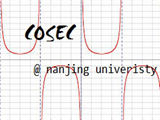
\includegraphics[height=1.5cm]{cosec.jpg}{\hspace{30pt}}}    % If you do not need logo, just comment out it


% ---------------- Document begins ----------------
\begin{document}

\setbeamertemplate{headline}[nju theme no tos]
\frame{\titlepage}

\nologo
\setbeamertemplate{headline}[nju theme]

\frame{\frametitle{目录}\tableofcontents}			

% Now followed blindtext, just for test
\section{Section 1}
\begin{frame}
  \frametitle{Section 1}

    In this slide, some important text will be
    \alert{highlighted} because it's important.
    Please, don't abuse it.

    \begin{block}{Remark}
      Sample text
    \end{block}

    \begin{alertblock}{Important theorem}
      Sample text in red box
    \end{alertblock}

    \begin{examples}
      Sample text in green box. The title of the block is ``Examples".
    \end{examples}

\end{frame}

\section{Section 2}
\begin{frame}[fragile]      % If you are using minted, remember to append fragile option to the frame
  \frametitle{Section 2}

    Houston, we have a problem.

    \vspace*{10pt}

    \begin{minted}[fontsize=\scriptsize]{java}
try {
    throw new Exception("blah");
} catch(Exception e) {
    for (StackTraceElement stackTraceElement: e.getStackTrace()) {
        // stackTraceElement.getClassName() stackTraceElement.getMethodName()
        // try to find Hook Frame in the calling stack
    }
}
    \end{minted}

    \blfootnote{\tiny \url{https://www.gutenberg.org/files/18269/18269-h/18269-h.htm\#p_347}}

\end{frame}

\section{Section 3}
\begin{frame}
  \frametitle{Section 3}
    \resizebox{4cm}{4cm}{%
      \sqrtspiral{10}
    }
~\vfill
    Example of pdfcomment
    \pdfcomment{
    blahblahblah, \textCR
    blahblah.}

\end{frame}

\subsection{Subsection 4}
\begin{frame}
  \frametitle{Subsection 4}

    Example of pdfnote
    \pdfnote{remember to say thankyou!!!}

\end{frame}

\setbeamertemplate{headline}[nju theme no tos] 
\begin{frame}
    \centering \Large Thanks for watching!
\end{frame}

% If needed
\setbeamertemplate{background}{\pgfuseimage{bg}}
\frame{\tableofcontents}

\end{document}
